\documentclass{article}
\usepackage{graphicx}
\usepackage{amsmath}
\usepackage{epsf}
\usepackage{systeme}  
\usepackage{xcolor}
\usepackage{float}
\usepackage{hyperref} 
% titlepage causes separate title page
% our latex is biased off 1in vertically and horizontally
\newtheorem{theorem}{Theorem}
\setlength{\topmargin}{0.1in}
\setlength{\oddsidemargin}{0in}
\setlength{\evensidemargin}{0in}
\setlength{\headheight}{0in}
\setlength{\headsep}{0in}
\setlength{\textheight}{9in}
\setlength{\textwidth}{6.5in}
% require that floats fill 90% of a page in order for that page to be
% ``float-only''
\renewcommand{\dblfloatpagefraction}{0.9}
\renewcommand{\floatpagefraction}{0.9}
%\renewcommand{\baselinestretch}{1.2} % interline spacing
%\setlength{\parindent}{0in}
%\parskip=10pt plus2pt minus2pt
%\setlength{\unitlength}{0.1in}
%\pagestyle{empty} % no page numbering
\newenvironment{bibparagraph}{\begin{list}{}{ %
    \setlength{\labelsep}{-\leftmargin} %
    \setlength{\labelwidth}{0pt} %
    \setlength{\itemindent}{-\leftmargin} %
    \setlength{\listparindent}{0pt}}}{\end{list}}
\def\makefigure#1#2{\begin{figure}
\begin{center}
\input{#1}
\end{center}
\caption{#2}
\label{#1}
\end{figure}}

\def\limplies{\; \supset \;}
\def\land{\: \wedge \:}
\def\lor{\: \vee \:}
\def\iff{\; \equiv \;}
\def\lnot{\neg}
\def\lforall#1{\forall \: #1 \;}
\def\lexists#1{\exists \: #1 \;}
\def\glitch#1{{\tt #1}} % glitch on
%\def\glitch#1{} % glitch off
\def\comment#1{}
\def\pnil{[\;]}
\def\pif{\; \mbox{\tt :- } \;}
\def\tuple#1{$\langle #1\rangle$}
\def\mtuple#1{\langle #1\rangle}
\def\ceiling#1{\lceil #1\rceil}
\def\floor#1{\lfloor #1\rfloor}
\def\centerps#1{\begin{center}
\leavevmode
\epsfbox{#1}
\end{center}}
\def\argmax{\mathop{\rm argmax}}
\def\argmin{\mathop{\rm argmin}}
\def\grad{\nabla\!}
\def\celsius{^\circ\mbox{C}}
%\long\def\answer#1{}  % comment out for solutions
%\long\def\question#1{#1} % comment out for solutions
\long\def\answer#1{{\color{blue}{\sl #1}}}  % comment in for solution
\long\def\question#1{} % comment in for solution
\renewcommand{\labelenumi}{(\alph{enumi})}

\def\x{{\bf x}}
\def\y{{\bf y}}
\def\w{{\bf w}}

\begin{document}
{\Large
\begin{center}
CS534 --- Written Homework Assignment 0 \\\answer{Your name goes here}
\end{center}
}
%Please submit electronically via TEACH in a single pdf file.
\section*{Linear algebra}

\begin{enumerate}
\item \textbf{Transpose and Associative Property, Positive Semi-definite matrices [2pt]}
Define a matrix $B = b{b^T}$, where $b \in \mathbf{R}^{d\times1}$ is a column vector that is not all-zero. Show that $B$ is a positive semi-definite matrix.\\

[\emph{Hint}: To show that $B$ is positive semi-definite, we need to show that $B$ is symmetric, and  for any vector $x\in \mathbf{R}^{d\times1}$, $x^TBx \geq 0$. For the latter, try to get $x^TBx$ to look like the product of two identical scalars. Note that $b^Tx = (x^Tb)^T$, that $a^T=a$ for scalar value $a$, and that matrix multiplication is associative.]\\
\answer{Your solution goes here.
}
\item \textbf{Solving systems of linear equations with matrix inverse. [2pt]} Consider the following set of linear equations:
    \begin{equation*}
    \systeme{
    x_1  + x_2 - x_3 - x_4  =1, 
    2x_1 + 5x_2- 7x_3- 5x_4 =-2, 
    2x_1 - x_2 + x_3 + 3x_4 =4, 
    5x_1 + 2x_2 - 4x_3- 2x_4 =6}        
    \end{equation*}
    
    \begin{enumerate}
        \item (1 pt) Please express the system of equations as $A\x={\bf b}$ by specifying the matrix $A$ and vector ${\bf b}$\\
        \answer{Your solution goes here.
        
        }

       
        \item (1 pt) Solve for $A\x={\bf b}$ by using the matrix inverse of $A$ (you can use software to compute the inverse).  \\
        \answer{Your solution goes here.}
    \end{enumerate}
\end{enumerate}

\section*{Vector Calculus}
\begin{enumerate}
    \item \textbf{Derivatives.[2pt]}. Compute the derivative $f'(x)$ for 
    \begin{enumerate}
        \item (1 pts) the logistic (aka sigmoid) function $f(x) = \frac{1}{1+\exp(-x)}$
        \\
        \answer{Your solution goes here.
        }
        \item (1 pts) $f(x) = \exp(-\frac{1}{2\sigma^2}(x-\mu)^2)$\\
        \answer{Your solution goes here.}
    \end{enumerate}
    \item \textbf{Gradients. [3pt]}Compute the gradient $\nabla_{\x}f$ of the following functions. Please clearly specify the dimension of the gradient. 
\begin{enumerate}
    \item (1pt) \[f(z)=\log(1+z)\mbox{,  }  z= \x^T\x\mbox{,  } \x\in R^D\] \\
\answer{Your solution goes here.}

    \item (2pt)  \[f(z) = \exp{(-\frac{1}{2}z)} \]
    \[ z=g(\y)=\y^T S^{-1}\y \]
    \[ \y=h(\x)= \x-\mathbf{\mu} \]
    \[\mbox{where } \mathbf{x}, \mathbf{\mu} \in R^D, S\in R^{D\times D} \mbox{ is a symmetric matrix.}\] 
    \\
\answer{Your solution goes here}
\end{enumerate}    


\end{enumerate}
\section*{Probability}
\begin{enumerate}
\item \textbf{Joint, Marginal, and Conditional Probabilities [2pt]} Consider two discrete random variables $X$ and $Y$ with the following joint distribution: 
\begin{figure*}[h]
    \centering
    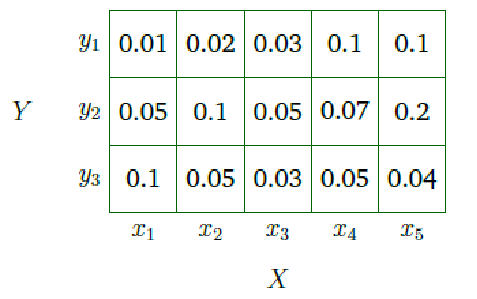
\includegraphics[width=3in]{joint.pdf}
\end{figure*}

Please compute: 
\begin{enumerate}
    \item (1 pt) The marginal distributions $p(x)$ and $p(y)$ \\
    \answer{Your solution goes here.
    }
    \item (1 pt)  The Conditional distribution $p(x|Y=y_1)$ and $p(y|X=x_3)$\\
    \answer{
Your solution goes here.}
\end{enumerate}
    
\item \textbf{Conditional probabilities, Marginalization and Bayes Rule [5pt]} Consider two coins, one is fair and the other one has a 1/10 probability for head. Now you randomly pick one of the coins, and toss it twice. Answer the following questions.
    \begin{enumerate}

    \item (1pt) What is the probability that you picked the fair coin? What is the probability of the first toss being head?\\
    \answer{Your solution goes here.}

    \item (2pts) If both tosses are heads, what is the probability that you have chosen the fair coin (Hint: you should apply Bayes Rule for this)?\\
    \answer{Your solution goes here.}

\item (2pts) If both tosses are heads, what is the probability that the third coin toss will be head? (you should build on results of b)\\
\answer{ Your solution goes here.
}
\end{enumerate}

\item \textbf{Linearity of Expectation [2 pt]} A random variable x distributed according to a standard normal distribution (mean zero and unit variance)
has the following probability density function (pdf):
%
\begin{align*}
p(x) = \frac{1}{{\sqrt {2\pi } }}{e^{ - \frac{{{x^2}}}{2}}}
\end{align*}
%
Using the properties of expectations, evaluate the following integral
%
\begin{align*}
\int\limits_{ - \infty }^\infty  {p(x)(a{x^2} + b{x} + c)dx}
\end{align*}

[\emph{Hint:} This is \emph{not} a calculus question. The simple solution relies on linearity of expectation and the provided mean/variance of p(x).]


\answer{Your solution goes here.}

\item \textbf{Cumulative Density Functions / Calculus [2 pt]}
$X$ is a continuous random variable over the interval [0,1], show that the following function $p$ is a valid probability density function (PDF) and derive the corresponding cumulative density function (CDF). %
\begin{align*}
p(x) = \left\{ {\begin{array}{*{20}{c}}
{\begin{array}{*{20}{c}}
{4x}&{0 \le x \le 1/2}
\end{array}}\\
{\begin{array}{*{20}{c}}
{ - 4x + 4}&{1/2 \le x \le 1}
\end{array}}
\end{array}} \right.
\label{eq:pdf}
\end{align*}
%

[\emph{Hint:} Recall that a function is a valid PDF function if it integrates to 1: $\int_{-\infty}^{\infty}~p(x)~dx=1$. And the cumulative density function (CDF) is defined as $C(x) = P(X \le x)$ or the probability that a sample from $p$ is less than $x$ -- which can be computed as $C(x) = \int_{-\infty}^x~p(x)~dx$.  This \emph{is} a calculus question. But the PDf is a piece-wise linear function, hence it is straightforward.]

\answer{Your solution goes here}


\end{enumerate}

\end{document}

